\documentclass[11pt,a4paper]{report}
\usepackage{amsmath}
\usepackage{amssymb}

\usepackage{graphicx}

\usepackage{listings}
\usepackage{color} %red, green, blue, yellow, cyan, magenta, black, white
\definecolor{mygreen}{RGB}{28,172,0} % color values Red, Green, Blue
\definecolor{mylilas}{RGB}{170,55,241}


\usepackage{graphicx}


\begin{document}
\begin{center}

\LARGE Mat-Inf4140 - Mandatory assignment 2
\\
Andreas Thune
\\
\LARGE
16.02.2016

\end{center}
\textbf{4.2.5}
\\
Assume that we want to interpolate a function using the points $\{ x_i\}_{i=1}^n$. The Lagrange basis is the defined by $$q_i(x) = \prod_{j\neq i} \frac{x-x_j}{x_i-x_j} $$ This means that $q_i(x_j) = \delta_{ij}$, which again means that interpolation polynomial of samplevalues $\{ f_i\}_{i=1}^n$ at points $x_i$ is $$p(x) = \sum_{i=1}^n f_iq_i(x)= \sum_{i=1}^n f_i\prod_{j\neq i} \frac{x-x_j}{x_i-x_j}$$ Now for the barycentric form we define $$\phi(x) = \prod_{i=1}^n x-x_i $$ this gives the form 
\begin{align}
p(x) = \phi(x)\sum_{i=1}^n f_i\frac{w_i}{x-x_i} 
\end{align}
where $$w_i = \prod_{j\neq i} \frac{1}{x_i-x_j}$$
We also see that the individual Lagrange polynomials can be written as $$l_j(x)=\phi(x)\frac{w_j}{x-x_j} $$ This helps us to get an alternative way of expressing the barycentric form, when we remember that the sum of all of the Lagrange polynomials equals 1. 
\begin{align*}
&1=\sum_{j=1}^n l_j(x)= \phi(x)\sum_{j=1}^n \frac{w_j}{x-x_j} \\
&\iff \phi(x) = \frac{1}{\sum_{j=1}^n \frac{w_j}{x-x_j}}
\end{align*} 
Putting the above expression into (1) gives us the following:
\begin{align*}
p(x)=\frac{\sum_{i=1}^n f_i\frac{w_i}{x-x_i}}{\sum_{j=1}^n \frac{w_j}{x-x_j}}
\end{align*}
The reason for using this barycentric form and not the original expression for the Lagrange interpolation polynomial, is to save computing time. For The barycentric form we need to compute weights $w_i$ for all i before we start evaluating our polynomial. This requires $O(n^2)$ FLOPS, but when we have computed this, it only takes $O(n)$ flops to evaluate our polynomial at any given value. This is not the case for our original expression, that requires $O(n^2)$ FLOPS for evaluation. 
\\
\textbf{4.3.2}
\\
Assume that we have a function $f$ and its derivative $f'$. Use Hermation interpolation to approximate f in the the two points $\{x_1,x_2\}$ by cubic polynomial $p$ such that the derivative of $p$ is equal to the derivative of $f$ in the points. If we choose the power basis, we want $$p(x)=c_0 + c_1x + c_2x^2 + c_3x^3$$ If we differentiate $p$ we get $$p'(x)=c_1 + 2c_2x + 3c_3x^2$$ We then get a system of eqation from the conditions $p(x_1)=f(x_1)=f_1$, $p'(x_1)=f'_1$, $p(x_2)=f_2$ and $p'(x_2)=f'_2$, were the $c_i$ coefficients are the unknowns. This gives us the system $Ac=b$, were c is: $$c=(c_0,c_1,c_2,c_3)^T$$ b is: $$b=(f_1,f'_1,f_2,f'_2)^T$$ and A is:  

$$ 
A = 
 \begin{pmatrix}
  1 & x_1 & x_1^2 &  x_1^3 \\
  0 & 1 & 2x_1 & 3x_1^2 \\
  1 & x_2 & x_2^2  & x_2^3  \\
  0 & 1 & 2x_2  & 3x_2^2 
 \end{pmatrix}
$$
\\
\\
\textbf{CE: 4.3.9}
\\
a) To show bilinear interpolation formula we need Taylor's formula:
\begin{align*}
f(x_0+ph,y_0+qk)&= f(x_0,y_0) + phf_x(x_0,y_0)+qkf_y(x_0,y_0)\\
&+qhphf_{xy}(x_0,y_0)+\frac{(ph)^2}{2}f_{xx}(x_0,y_0)+\frac{(qk)^2}{2}f_{yy}(x_0,y_0) +O(h^3+k^3)
\end{align*}
We want estimate $f$ derivatives using the points $(x_0,y_0)$,$(x_0+h,y_0)$,$(x_0,y_0+k)$ and $(x_0+h,y_0+k)$. From now on evaluating at these points will be written $f_{00}$, $f_{10}$, $f_{01}$ and $f_{11}$. We now estimate the derivatives using finite difference. We also ignore the $f_{xx}$ and $f_{yy}$ terms. This gives us 
\begin{align*}
r(p,q)&=f_{00} +ph\frac{f_{10}-f_{00}}{h}+qk\frac{f_{00}-f_{00}}{k} +phqk(\frac{f_{10}-f_{00}}{h})_y \\
&=(1-p-q)f_{00} + pf_{10}+qf_{01} +pqk(\frac{f_{11}-f_{10}}{k}-\frac{f_{01}-f_{00}}{k}) \\
&= (1-p-q+pq)f_{00} +(p-pq)f_{10}+(q-pq)f_{01}+ pqf_{11} \\
&=(1-p)(1-q)f_{00}+p(1-q)f_{10}+q(1-p)f_{01}+ pqf_{11}
\end{align*} 
Note that when we do finite difference to approximate a derivative of a function $g$, we make an error that looks like this:
\begin{align*}
E(x)=\frac{g(x+h)-g(x)}{h}-g'(x) = \frac{h}{2}g''(x) + O(h^2)
\end{align*} 
This means that we get following error from our approximation function $r$:
\begin{align*}
E(p,q) = \frac{1}{2}(ph^2f_{xx}(x_0,y_0)+qk^2f_{yy}(x_0,y_0)) +O(h^3+k^3+(hk)^2) 
\end{align*}
Here I will just assume that the error from finite differencing a term in two directions gives the errors multiplied with each other. our expression $r$ is the expression we want to get. Now lets try to get the same error estimate as they got in the book. First define $s(p,q)$:
\begin{align*}
s(p,q)= f_{00} +ph\frac{f_{10}-f_{00}}{h}+qk\frac{f_{00}-f_{00}}{k} +phqk(\frac{f_{10}-f_{00}}{h})_y
\end{align*}
We then have that $r(p,q)-s(p,q)=E(p,q)$. This gives us:
\begin{align*}
|r(p,q)-f(x_0+ph,y_0+qk)| = &|r(p,q)-s(p,q)+s(p,q)-f(x_0+ph,y_0+qk)| \\
=&|E(p,q)+s(p,q)-f(x_0+ph,y_0+qk)| \\
=&|\frac{1}{2}(ph^2f_{xx}(x_0,y_0)+qk^2f_{yy}(x_0,y_0)) +O(h^3+k^3+(hk)^2)\\
&-(\frac{(ph)^2}{2}f_{xx}(x_0,y_0)+\frac{(qk)^2}{2}f_{yy}(x_0,y_0) +O(h^3+k^3))| \\
\leq &\frac{1}{2}(p(1-p)h^2|f_{xx}|+q(1-q)k^2|f_{yy}|)+ O((hk)^2)
\end{align*}
here $|f_{xx}|$ and $|f_{yy}|$ is the max norm of those two functions. This is what we wanted.
\\
\\
b) This is a trivial exercise, everything is in the code.
\\
\\
\textbf{CE: 4.3.12}
\\
a) We want to interpolate the function $f(x)=cot(x)$ at five points using rational interpolation of order (2,2). This means that we want to find two second order polynomials $p$ and $q$ such that $$\frac{p(x_i)}{q(x_i)}=f(x_i) $$ for $i=1,2,3,4,5$. We define $p$ and $q$ as: 
\begin{align*}
p(x) &= c_0+c_1x+c_2x^2 \\
q(x) &= d_0+d_1x+d_2x^2
\end{align*} 
To solve this we change the problem to $$p(x_i)-f(x_i)q(x_i)=0$$ This gives us the following system: 
\begin{align*}
Ac-FBd=0
\end{align*}
were $c=(c_0,c_1,c_2)$,  $d=(d_0,d_1,d_2)$, F is a diagonal matrix with $f_i$ at its diagonal,
$$ 
A = 
 \begin{pmatrix}
  1 & x_1 & x_1^2  \\
  1 & x_2 & x_2^2  \\
  1 & x_3 & x_3^2   \\
  1 & x_4 & x_4^2 \\
  1 & x_5 & x_5^2
 \end{pmatrix}
$$
and 
$$ 
B = 
 \begin{pmatrix}
  f_1 & f_1x_1 & f_1x_1^2  \\
  f_2 & f_2x_2 & f_2x_2^2  \\
  f_3 & f_3x_3 & f_3x_3^2   \\
  f_4 & f_4x_4 & f_4x_4^2 \\
  f_5 & f_5x_5 & f_5x_5^2
 \end{pmatrix}
$$
This system can be rewritten to $$Ey=0$$ where $y = (c_0,c_1,c_2,d_0,d_1,d_2)$ and 
$$
E = 
 \begin{pmatrix}
  1 & x_1 & x_1^2 & -f_1 & -f_1x_1 & -f_1x_1^2  \\
  1 & x_2 & x_2^2 & -f_2 & -f_2x_2 & -f_2x_2^2  \\
  1 & x_3 & x_3^2 & -f_3 & -f_3x_3 & -f_3x_3^2   \\
  1 & x_4 & x_4^2 & -f_4 & -f_4x_4 & -f_4x_4^2 \\
  1 & x_5 & x_5^2 & -f_5 & -f_5x_5 & -f_5x_5^2
 \end{pmatrix}
$$
This system has six unknowns and five equations, and is therefore not uniquely solvable. To find a solution, I will do as described in an example in the book, and just say that $c_2=1$. This will then give us yet another system $$Qz=-x^2$$ Where $z$ is y without $c_2$, $-x^2$ is our five points squared, and 
$$
Q = 
 \begin{pmatrix}
  1 & x_1 &  -f_1 & -f_1x_1 & -f_1x_1^2  \\
  1 & x_2 &  -f_2 & -f_2x_2 & -f_2x_2^2  \\
  1 & x_3 &  -f_3 & -f_3x_3 & -f_3x_3^2   \\
  1 & x_4 &  -f_4 & -f_4x_4 & -f_4x_4^2 \\
  1 & x_5 &  -f_5 & -f_5x_5 & -f_5x_5^2
 \end{pmatrix}
$$
This system can be solved and solving this system is exactly what I have done in the code. The code can be found below.
\\
\\
b) In this exercise we were asked to interpolate $cot(x)$ using normal polynomial interpolation. I will not describe how to find the linear system, but what I did is in the code below. We were also asked to comment an the difference between the result of the polynomial and rational interpolation. The exercise asked for the error between the exact and the two types of interpolation in $x=2.5^o$. The result of this was $error\approx2.6e-8 $ for rational and $error\approx2.7 $ for normal polynomial. The difference in the error between the two methods was in this case a factor of $10^{-8}$. This is allot, and I think that the reason the rational interpolation is so good in this case is that $½cot(x)$ blows up at $x=0$, which is a feature that can be replicated for rational functions, but not for polynomials. To underline the difference between the two methods even more I have included a plot that shows what happens when the function values are not in $[1^o,5^o]$.

\begin{figure}
  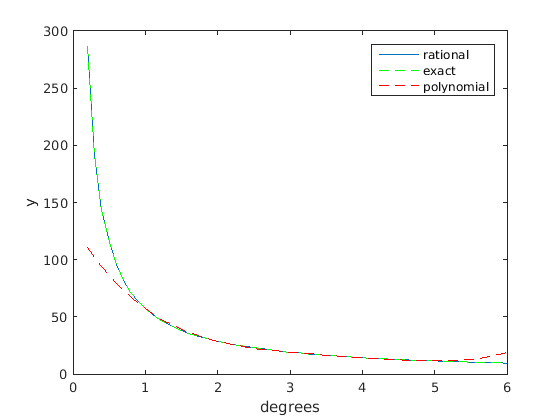
\includegraphics[width=\linewidth]{oblig2_rational.png}
  \caption{plot of $cot(x)$,rational and polynomial interpolation}
  \label{Fig 1}
\end{figure}

\lstset{language=Matlab,%
    %basicstyle=\color{red},
    breaklines=true,%
    morekeywords={matlab2tikz},
    keywordstyle=\color{blue},%
    morekeywords=[2]{1}, keywordstyle=[2]{\color{black}},
    identifierstyle=\color{black},%
    stringstyle=\color{mylilas},
    commentstyle=\color{mygreen},%
    showstringspaces=false,%without this there will be a symbol in the places where there is a space
    numbers=left,%
    numberstyle={\tiny \color{black}},% size of the numbers
    numbersep=9pt, % this defines how far the numbers are from the text
    emph=[1]{for,end,break},emphstyle=[1]\color{red}, %some words to emphasise
    %emph=[2]{word1,word2}, emphstyle=[2]{style},    
}
\section*{Code for Bilinear interpolation formula 4.3.9}
\lstinputlisting{oblig2/bilinear_inter.m}


\section*{Code for 4.3.12. Rational and polynomial interpolation}
\lstinputlisting{oblig2/rational.m}


\end{document}